\documentclass{article}

\usepackage{enumitem}
\usepackage{fontspec}
\usepackage[letterpaper,margin=72pt]{geometry}
\usepackage{hyperref}
\usepackage{import}
\usepackage{listings}
\usepackage{xcolor}

\subimport{../}{colors.tex}

\setsansfont{Overpass}[Scale=MatchLowercase]
\setmonofont{Overpass Mono}[Scale=MatchLowercase]

\renewcommand{\familydefault}{\sfdefault}

\hypersetup{
  colorlinks=true,
  urlcolor=uclablue,
}

\setlist{nosep}

\makeatletter
\newcommand\version[1]{\renewcommand\@version{#1}}
\newcommand\@version{}

\newcommand\labnumber[1]{\renewcommand\@labnumber{#1}}
\newcommand\@labnumber{}

\newcommand\duedate[1]{\renewcommand\@duedate{#1}}
\newcommand\@duedate{}

\renewcommand\maketitle{%
  \noindent
  {\Large \color{uclablue} CS 111: Operating System Principles}

  \noindent
  {\Large \color{uclablue} Lab \@labnumber}\\[-0.75em]

  \noindent
  {\Huge \bfseries \color{uclablue} \@title}
  {\ttfamily \footnotesize \color{uclablue} \@version}\\[-0.75em]

  \noindent
  {\@author}

  \noindent
  {\@date}

  \noindent
  {Due: \@duedate}\\[1em]
}
\makeatother

\lstset{
  basicstyle=\ttfamily,
}


\lecturenumber{1}
\title{Overview}
\version{2.0.0}
\author{Jon Eyolfson}
\date{June 22, 2021}

\begin{document}

  \begin{frame}[plain, noframenumbering]
    \titlepage
  \end{frame}
  
  \begin{frame}
    \vfill
    ``All problems in computer science can be solved by another level of
    indirection''

    \begin{flushright}
      - David Wheeler
    \end{flushright}
    \vfill
  \end{frame}

  \begin{frame}
    \frametitle{An Operating System Sits between Applications and Hardware}

    \centering
    \begin{tikzpicture}[every node/.style={draw, minimum width=4cm, inner sep=0.5em}]
      \node (app) {Application};
      \node [below=of app] (os) {Operating System};
      \node [below=of os] (hw) {Hardware};

      \draw [->, transform canvas={xshift=-3mm}] (app) -- (os);
      \draw [->, transform canvas={xshift=3mm}] (os) -- (app);

      \draw [->, transform canvas={xshift=-3mm}] (os) -- (hw);
      \draw [->, transform canvas={xshift=3mm}] (hw) -- (os);
    \end{tikzpicture}

    \begin{flushright}
      The primary role of an operating system is to manage and coordinate resources
    \end{flushright}
  \end{frame}

  \begin{frame}
    \frametitle{Ubuntu and Android are Considered Different Operating Systems}

    Both use a Linux kernel, but they run different applications

    \vspace{2em}

    There isn't a clear line, especially with ``Linux''

    \vspace{4em}

    For desktop applications, you'd draw the line at the Display System

    \vspace{2em}

    ``Linux'' uses Wayland, and Android uses SurfaceFlinger
  \end{frame}

  \begin{frame}
    \frametitle{Operating Systems Allow Running More than One Application}

    Without an operating system, a CPU starts executing code at a fixed address

    \vspace{4em}

    You could put your application here, but it would be the only one

    \vspace{2em}

    You would have to handle specific hardware in your application

    \vspace{4em}

    Instead, we start executing an operating system at boot
  \end{frame}

  \begin{frame}
    \frametitle{Our First Abstraction is a Process}

    Each process contains its own set of registers, including the program counter

    \vspace{2em}
    
    When starting a process, it specifies where the CPU should start executing

    \vspace{4em}

    The operating systems has to:
    \begin{itemize}
      \item Keeps track of registers for each process
      \item Switch between different processes
      \item Decide when to switch between processes
    \end{itemize}
  \end{frame}

  \begin{frame}
    \frametitle{We Could Put Applications in Different Parts of Memory}

    \centering
    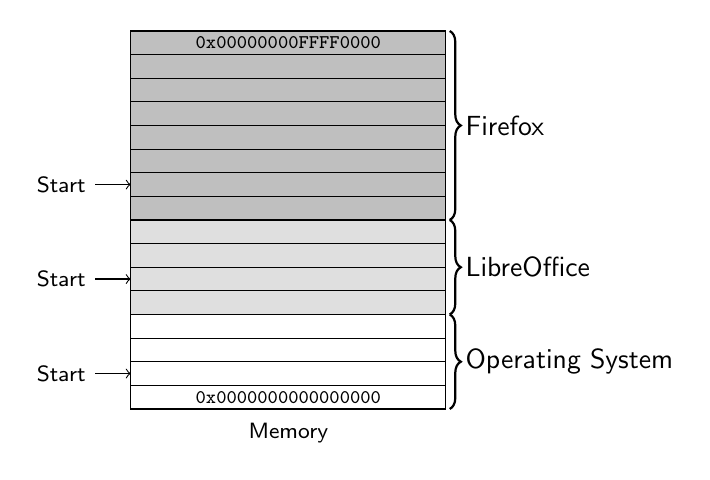
\begin{tikzpicture}
      \node [align=center] at (2, 0) {\footnotesize Memory};
      \draw [fill=black!25] (0, 2.7) rectangle (4, 5.1);
      \draw [fill=black!12.5] (0, 1.5) rectangle (4, 2.7);
      \node [align=center] at (2, 0.45) {\scriptsize \ttfamily 0x0000000000000000};
      \node [align=center] at (2, 4.95) {\scriptsize \ttfamily 0x00000000FFFF0000};
      \foreach \i in {1, ..., 16}
      {
        \draw (0, 0.3 * \i) rectangle (4, \i * 0.3 + 0.3);
      }
      \draw [decorate, decoration={brace, amplitude=4pt, mirror}, thick]
        (4.05, 0.3) -- (4.05, 1.5) node [midway, anchor=west, xshift=0.2em]
        {Operating System};
      \draw [decorate, decoration={brace, amplitude=4pt, mirror}, thick]
        (4.05, 1.5) -- (4.05, 2.7) node [midway, anchor=west, xshift=0.2em]
        {LibreOffice};
      \draw [decorate, decoration={brace, amplitude=4pt, mirror}, thick]
        (4.05, 2.7) -- (4.05, 5.1) node [midway, anchor=west, xshift=0.2em]
        {Firefox};

      \draw [->] (-0.45, 0.75) -- (0, 0.75) node [pos=0, anchor=east] {\footnotesize Start};
      \draw [->] (-0.45, 1.95) -- (0, 1.95) node [pos=0, anchor=east] {\footnotesize Start};
      \draw [->] (-0.45, 3.15) -- (0, 3.15) node [pos=0, anchor=east] {\footnotesize Start};
    \end{tikzpicture}

    \begin{flushright}
      This isn't very flexible
    \end{flushright}
  \end{frame}

  \begin{frame}
    \frametitle{Virtualization Fools Something into Thinking it Has All Resources}

    \begin{columns}[c]
      \column{0.5\textwidth}
      \flushright
    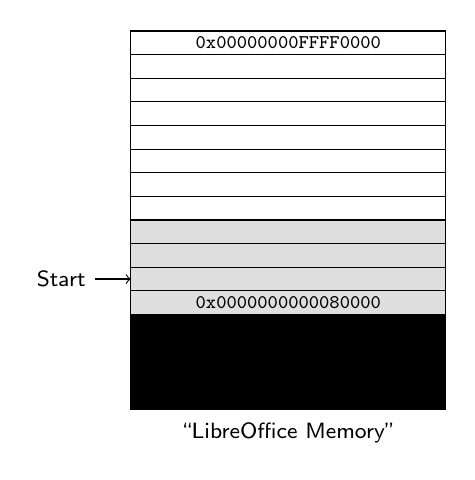
\begin{tikzpicture}
      \node [align=center] at (2, 0) {\footnotesize ``LibreOffice Memory''};
      \draw [fill=black] (0, 0.3) rectangle (4, 1.5);
      \draw [fill=black!12.5] (0, 1.5) rectangle (4, 2.7);
      \node [align=center] at (2, 1.65) {\scriptsize \ttfamily 0x0000000000080000};
      \node [align=center] at (2, 4.95) {\scriptsize \ttfamily 0x00000000FFFF0000};
      \foreach \i in {1, ..., 16}
      {
        \draw (0, 0.3 * \i) rectangle (4, \i * 0.3 + 0.3);
      }

      \draw [->] (-0.45, 1.95) -- (0, 1.95) node [pos=0, anchor=east] {\footnotesize Start};
    \end{tikzpicture}
      \column{0.5\textwidth}
      \flushleft
    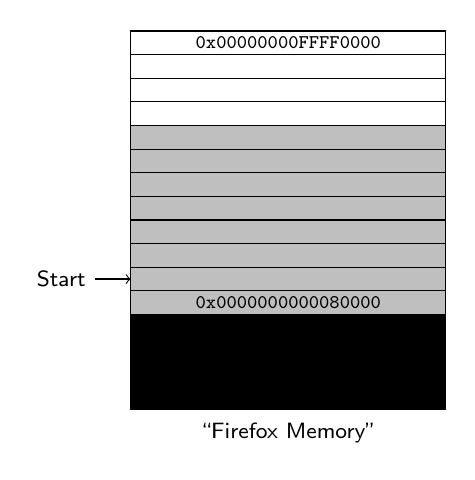
\begin{tikzpicture}
      \node [align=center] at (2, 0) {\footnotesize ``Firefox Memory''};
      \draw [fill=black] (0, 0.3) rectangle (4, 1.5);
      \draw [fill=black!25] (0, 1.5) rectangle (4, 3.9);
      \node [align=center] at (2, 1.65) {\scriptsize \ttfamily 0x0000000000080000};
      \node [align=center] at (2, 4.95) {\scriptsize \ttfamily 0x00000000FFFF0000};
      \foreach \i in {1, ..., 16}
      {
        \draw (0, 0.3 * \i) rectangle (4, \i * 0.3 + 0.3);
      }

      \draw [->] (-0.45, 1.95) -- (0, 1.95) node [pos=0, anchor=east] {\footnotesize Start};
    \end{tikzpicture}
    \end{columns}
  \end{frame}

  \begin{frame}
    \frametitle{Virtual Memory Abstracts Away Physical Memory}

    Each process believes it has access to all the memory

    \vspace{2em}

    Different processes can have the same starting address


    \vspace{4em}

    The operating system has to:
    \begin{itemize}
      \item Map virtual memory access to physical memory
      \item Keep track of memory usage (allocate and deallocate)
      \item Handle out-of-memory scenarios
    \end{itemize}
  \end{frame}

  \begin{frame}
    \frametitle{Virtualization is a Powerful Concept}

    Applies to both processes and virtual memory

    \vspace{4em}

    We can extend this to an entire machine

    \vspace{2em}

    A single physical machine can run multiple operating systems at once
  \end{frame}

  \begin{frame}
    \frametitle{Concurrency is Multiple Things Happening at the Same Time}

    We want multiple applications running at once

    \vspace{2em}

    We want applications to do multiple things at once

    \vspace{4em}

    We don't want applications isolated

    \vspace{2em}

    We want applications and libraries to communicate   
  \end{frame}

  \begin{frame}
    \frametitle{Concurrency is Necessary for Operating Systems}

    Running one application at a time isn't a good experience

    \vspace{2em}

    Completely isolated applications aren't useful

    \hspace{2em} The simplest applications still communicate with the terminal

    \vspace{4em}

    The operating system has to:
    \begin{itemize}
      \item Allow multiple executions at once, safely
      \item Manage abstractions for different kinds of inter-process communication (IPC)
      \item Provide permission checking and access control
    \end{itemize}
  \end{frame}

  \begin{frame}
    \frametitle{Finally, We Need Persistence for a Basic Operating System}

    We want to be able to access data between boots

    \vspace{2em}

    A file system specifies how to organize data on a storage medium

    \vspace{4em}
    
    The operating system has to:
    \begin{itemize}
      \item Store and retrieve data
      \item Ensure integrity of data
    \end{itemize}
  \end{frame}

  \begin{frame}
    \frametitle{File Descriptors Abstract Both Communication and Persistence}

    A file descriptor is just a number identifier (per process) that you can:
    \begin{itemize}
      \item Read bytes from
      \item Write bytes to 
    \end{itemize}

    \vspace{4em}

    The operating system can direct the bytes to whatever it represents

    \vspace{2em}

    You could imagine it representing a file, or one side of communication
  \end{frame}

  \begin{frame}
    \frametitle{Security is Another Consideration}

    We want our computers to only do what we tell them to

    \vspace{4em}

    The operating system has to:
    \begin{itemize}
      \item Encrypt of sensitive data
      \item Prevent bypassing access control
      \item Only execute applications the user wants
    \end{itemize}
  \end{frame}

  \begin{frame}
    \frametitle{Most Kernel Code is Device Drivers}

    Device drivers implement the abstractions we'll learn to the physical hardware

    \vspace{2em}

    It involves reading manufacturer specifications, and finding bugs

    \vspace{2em}

    Sometimes there's inconsistencies between documentation and reality
  \end{frame}

  \begin{frame}[fragile]
    \frametitle{An Actual Comment Linux Source (\texttt{arch/x86/kernel/apm\_32.c})}
    \begin{lstlisting}
/*
 *  Check for clue free BIOS implementations who use
 *  the following QA technique
 *
 *      [ Write BIOS Code ]<------
 *               |                ^
 *      < Does it Compile >----N--
 *               |Y               ^
 *      < Does it Boot Win98 >-N--
 *               |Y
 *           [Ship It]
 *
 *      Phoenix A04  08/24/2000 is known bad (Dell Inspiron 5000e)
 *      Phoenix A07  09/29/2000 is known good (Dell Inspiron 5000)
 */
    \end{lstlisting}
  \end{frame}

  \begin{frame}
    \frametitle{Believe It or Not, This Is ``Hello World''}

    \scriptsize \ttfamily
    0x7F 0x45 0x4C 0x46 0x02 0x01 0x01 0x03 0x00 0x00 0x00 0x00 0x00 0x00 0x00
    0x00

    0x02 0x00 0x3E 0x00 0x01 0x00 0x00 0x00 0x78 0x00 0x01 0x00 0x00 0x00 0x00
    0x00

    0x40 0x00 0x00 0x00 0x00 0x00 0x00 0x00 0x00 0x00 0x00 0x00 0x00 0x00 0x00
    0x00

    0x00 0x00 0x00 0x00 0x40 0x00 0x38 0x00 0x01 0x00 0x40 0x00 0x00 0x00 0x00
    0x00

    0x01 0x00 0x00 0x00 0x05 0x00 0x00 0x00 0x00 0x00 0x00 0x00 0x00 0x00 0x00
    0x00

    0x00 0x00 0x01 0x00 0x00 0x00 0x00 0x00 0x00 0x00 0x01 0x00 0x00 0x00 0x00
    0x00

    0xB2 0x00 0x00 0x00 0x00 0x00 0x00 0x00 0xB2 0x00 0x00 0x00 0x00 0x00 0x00
    0x00

    0x00 0x01 0x00 0x00 0x00 0x00 0x00 0x00 0x48 0xC7 0xC0 0x01 0x00 0x00 0x00
    0x48

    0xC7 0xC7 0x01 0x00 0x00 0x00 0x48 0xC7 0xC6 0xA6 0x00 0x01 0x00 0x48 0xC7
    0xC2

    0x0C 0x00 0x00 0x00 0x0F 0x05 0x48 0xC7 0xC0 0xE7 0x00 0x00 0x00 0x48 0xC7
    0xC7

    0x00 0x00 0x00 0x00 0x0F 0x05 0x48 0x65 0x6C 0x6C 0x6F 0x20 0x77 0x6F 0x72
    0x6C

    0x64 0x0A
  \end{frame}

  \begin{frame}
    \frametitle{There are 3 Major Concepts in This Course}

    You'll learn how the following applies to operating systems:
    \begin{itemize}
      \item Virtualization
      \item Concurrency
      \item Persistence
    \end{itemize}
  \end{frame}
\end{document}
